\chapter{Módulo de controle de infusão de insulina}
Este travalho tem o objetivo de estudar e desenvolver um protótipo do módulo de controle da bomba de infusão de insulina, para o desenvolvimento vamos utilizar o microcontrolado PIC18F452. Módulo este responsável por controlar o funcionamento da bomba em função dos parâmetros recebidos e pré estabelecidos. É possível configurar a quantidade a ser infundido no periodo de 24 horas, infusão basal, e, além disso e mais importante, o desenvolvimento foi feito em cima do simulador proteus e devido a possibilidade de mudanças possíveis o sistema foi montado de forma que deixa os módulos desacoplados. Para isso foi utilizado o conceito OOC, \emph{Object Orientated Programming in ANSI-C}, o que possibilitou o uso de \emph{Design Patterns}.

\section{\emph{OOC - \emph{Object Orientated Programming in ANSI-C}}}
Segudno \cite{schreiner1993object}, programação orientada a objetos é a atual "cura pra tudo", embora tenha sido em torno de muito mais de vinte anos. No fundo, talvez seja, um pouco mais do que isso, uma vez que finalmente aplica-se os bons princípios de programação que foi ensinado por mais de 30 anos. C + +, java, python, qualquer outra linguagem que seja escolhida são os "novos idiomas" da programação e isso porque são orientadas a objetos, embora não seja preciso utilizá-las, pois é possível fazer exatamente o mesmo com simples ANSI-C. Só orientação a objetos permite a reutilização de código entre os projetos, embora a idéia de funções é tão antiga quanto os computadores e desde sempre bons programadores faziam uso de ferramentas e bibliotecas prontas, as vezes desenvolvidas por eles mesmo.

A ideia de OOC é simplesmente mostrar como a programação orientada a objetos é feita e porque nos ajuda a resolver problemas maiores, aproveitando generalidade e encontrar erros mais cedos. Além de que saber utilizar isso na forma crua faz com que o entendimento de linguagens mais alto nivel desse paradigma se torne análoga e mais clara.

\section{\emph{Design Patterns}}
Na engenharia de \emph{software}, um \emph{Design Patterns} ou padrão de projeto é uma solução repetível geral para um problema comumente ocorre em \emph{design} de \emph{software}. Um padrão de projeto não é um projeto acabado que pode ser transformado diretamente em código. É uma descrição ou modelo de como resolver um problema que pode ser utilizado em diversas situações diferentes. \cite{shalloway2004design}.

\subsection{Usos de \emph{Design Patterns}}

Os \emph{Design Patterns} podem acelerar o processo de desenvolvimento, fornecendo testados e comprovados paradigmas de desenvolvimento. O \emph{design} de \emph{software} eficaz requer considerar as questões que não podem tornar-se visível até mais tarde na implementação. Reutilizar \emph{Design Patterns} ajuda a prevenir situações que podem causar grandes problemas e melhora a legibilidade do código para programadores e arquitetos familiarizados com os padrões.

Muitas vezes, as pessoas só entendem como aplicar certas técnicas de \emph{design} de \emph{software} para determinados problemas. Estas técnicas são difíceis de aplicar a uma ampla gama de problemas. Os \emph{Design Patterns} fornecem soluções gerais, documentadas em um formato que não requer especificidades ligadas a um problema particular \cite{shalloway2004design}.

Segundo \cite{shalloway2004design}, além disso, os padrões permitem que os desenvolvedores se comuniquem usando nomes bem conhecidos e bem compreendidos para interações de software. \emph{Design Patterns} comuns podem ser melhorados ao longo do tempo, tornando-os mais robustos do que os projetos ad-hoc, ou seja, problemas específicos. Os \emph{Design Patterns} podem ser divididos em:

\begin{itemize}
\item \emph{Creational design patterns}: Estes \emph{Design Patterns} tem tudo a ver com padrões de instanciação de classe. Esse padrão pode ser dividido em padrões de criação de classe e de criação de objetos. Enquanto os padrões de criação de classe usam a herança de forma eficaz no processo de instanciação, os padrões de criação de objeto usam a delegação de forma eficaz para ter o trabalho de criação feito. 
\item \emph{Structural design patterns}: Este \emph{Design Pattern} tem tudo a ver com composição de classe e objetos. Padrão estrutural de classe usa a herança para compor interfaces. Padrão estrutural de objeto define formas de compor objetos para obter novas funcionalidades.
\item \emph{Behavioral design patterns}: São os padrões que são mais especificamente relacionadas com a comunicação entre objetos.
\end{itemize}

\subsection{\emph{Factory Method}}
Segundo \cite{shalloway2004design}, \emph{factory method} foi um dos \emph{Design Patterns} escolhidos para esse projeto. Seus objetivos principais são:

\begin{itemize}
\item Definir uma interface para criar um objeto, mas deixa as subclasses decidirem qual classe instanciar. Factory Method permite adiar a instanciação da classe para a subclasses;
\item Definir um construtor \emph{virtual};
\item Operador \emph{new} é considerado perigoso.
\end{itemize}

Esse \emph{Design Patterns} foi utilizado no módulo que faz uso do \emph{display} de LCD para que a troca de seu tipo ficasse isolado do restante do sistema e que um futura troca possa ser feita com o menor impacto possível. A Figura \ref{fig:factorymethod} representa sua etsrutura em UML.

\begin{figure}[htp]
	\centering
	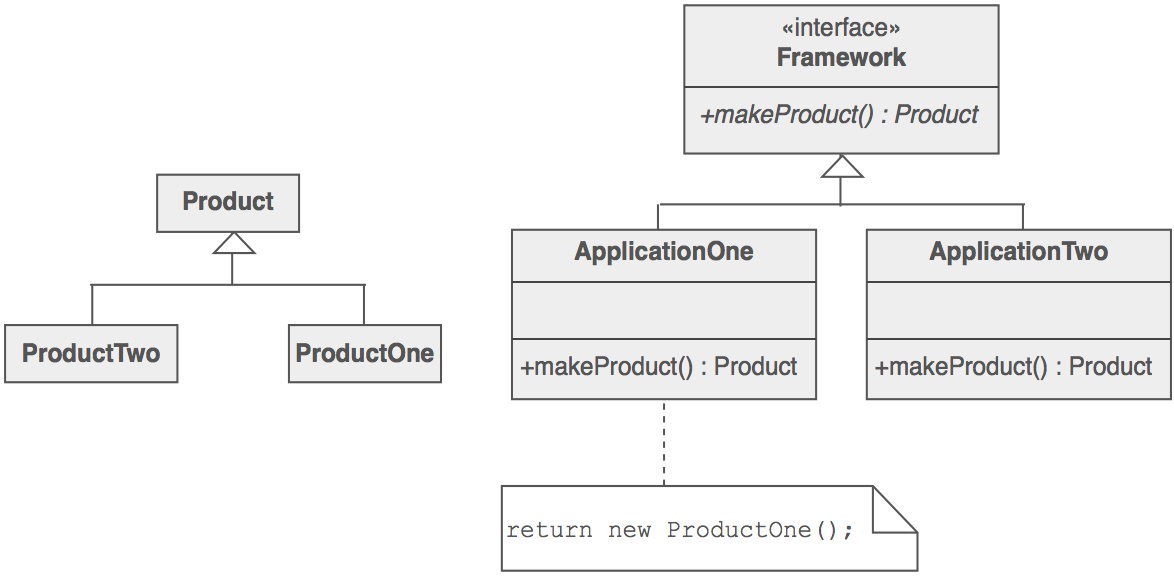
\includegraphics[scale=0.4]{images/Factory_Method.png}
	\caption{Estrutura do padrão \emph{Factory Method}}	
	\label{fig:factorymethod}
	\cite{shalloway2004design}
\end{figure}